\documentclass[11pt]{beamer}
\usetheme{simple}
\setbeamertemplate{footline}{} 
\usepackage{tikz, pgfplots,amsmath, amssymb, amsthm}   
\usepgfplotslibrary{groupplots}

\usepackage{sansmathaccent}
\pdfmapfile{+sansmathaccent.map}


%\pgfplotsset{ every non boxed y axis/.append style={y axis line style=-}}
\setbeamertemplate{navigation symbols}{}
\begin{document}
\begin{frame}




\only<1>{

\tikzset{every picture/.style={line width=0.75pt}} %set default line width to 0.75pt        

\begin{tikzpicture}[x=0.6pt,y=0.6pt,yscale=-1,xscale=1]
%uncomment if require: \path (0,443); %set diagram left start at 0, and has height of 443


/*!)-*&~n/{"isRoot":true,"isTextMode":true,"isTabularCellsSelected":false,"isPureText":false,"insideInlineMath":false,"lines":[{"blocks":[{"text":"\\diagram","type":"composite","elements":{},"connections":[],"intersections":{"id":"di19324905811464","items":[],"style":{}},"shapes":[{"id":"da3880007464371613","data":[{"x":47,"y":398},{"x":582,"y":398}],"head":"no","tail":"no","shaft":"."}],"settings":{"grid":false,"diagramHeight":492}}]}],"rootEditorId":"r0.9613564262074074","inlineMathDisplayStyle":null}

%Supply & Demand
\draw [color={rgb, 255:red, 245; green, 166; blue, 35 }  ,draw opacity=1 ][line width=2.25]    (126.5,361) -- (434.5,57) ;
\draw [color={rgb, 255:red, 74; green, 144; blue, 226 }  ,draw opacity=1 ][line width=2.25]    (124.28,83.03) -- (429.28,381.03) ;

%AXES
\draw  (74,382.93) -- (586.09,382.93)(125.21,36.6) -- (125.21,421.41) (579.09,377.93) -- (586.09,382.93) -- (579.09,387.93) (120.21,43.6) -- (125.21,36.6) -- (130.21,43.6)  ;
Straight Lines [id:da1654344051931811] 



%Equilibrium Point
\draw  [draw opacity=0][fill={rgb, 255:red, 0; green, 0; blue, 0 }  ,fill opacity=1 ] (263.97,222.35) .. controls (263.97,220.32) and (265.61,218.67) .. (267.65,218.67) .. controls (269.68,218.67) and (271.33,220.32) .. (271.33,222.35) .. controls (271.33,224.39) and (269.68,226.03) .. (267.65,226.03) .. controls (265.61,226.03) and (263.97,224.39) .. (263.97,222.35) -- cycle ;

%Straight line: EQ price
\draw  [dash pattern={on 0.84pt off 2.51pt}]  (124.5,222) -- (441.5,222) ;


%Straight Lines: EQ quanitity
\draw  [dash pattern={on 0.84pt off 2.51pt}]  (267.65,393) -- (267.65,222.35) ;


%Consumer Surplus
% \draw  [draw opacity=0][fill={rgb, 255:red, 74; green, 144; blue, 226 }  ,fill opacity=0.15 ] (124.28,83.03) -- (263.97,222.35) -- (124.28,222.35) -- cycle ;

%Shape: Producer Surplus
%\draw  [draw opacity=0][fill={rgb, 255:red, 0; green, 0; blue, 0 }  ,fill opacity=0.5 ] (267.18,224.07) -- (234.08,254.31) -- (235.65,192) -- cycle ;

%Deadweight Loss
%\draw  [draw opacity=0][fill={rgb, 255:red, 245; green, 166; blue, 35 }  ,fill opacity=0.15 ] (124.43,363) -- (267.5,222.35) -- (124.43,222.35) -- cycle ; \draw    (270.5,153) -- (245,219) ;\draw (275,137) node  [align=left] {Deadweight Loss};



%Shifted Demand
%\draw [color={rgb, 255:red, 74; green, 144; blue, 226 }  ,draw opacity=1 ][line width=2.25]  [dash pattern={on 2.53pt off 3.02pt}]  (124.28,143.03) -- (364.25,383) ;


%Straight Lines: Shifted EQ quantity
%\draw  [dash pattern={on 0.84pt off 2.51pt}]  (235.65,389) -- (235.65,254.35) ;
%\draw  [dash pattern={on 0.84pt off 2.51pt}]  (235.65,254.35) -- (235.65,192) ;

%Shifted Eq price: Consumer & Supplier
%\draw [shift={(235.65,192)}, rotate = 270] [color={rgb, 255:red, 0; green, 0; blue, 0 }  ][fill={rgb, 255:red, 0; green, 0; blue, 0 }  ][line width=0.75]      (0, 0) circle [x radius= 3.35, y radius= 3.35]   ;
%\draw [shift={(235.65,254.35)}, rotate = 270] [color={rgb, 255:red, 0; green, 0; blue, 0 }  ][fill={rgb, 255:red, 0; green, 0; blue, 0 }  ][line width=0.75]      (0, 0) circle [x radius= 3.35, y radius= 3.35]   ;

%Shape: Brace Taxes-- \draw   (123,85) .. controls (118.33,84.89) and (115.94,87.16) .. (115.83,91.83) -- (115.5,105.33) .. controls (115.33,112) and (112.92,115.27) .. (108.25,115.16) .. controls (112.92,115.27) and (115.17,118.66) .. (115.01,125.32)(115.08,122.33) -- (114.67,138.83) .. controls (114.56,143.5) and (116.83,145.89) .. (121.5,146) ;\draw (87,113) node   {$\text{tax} \ t$};

%Straight Lines: shifted Eq price, consumer -- \draw  [dash pattern={on 0.84pt off 2.51pt}]  (120.5,192) -- (235.65,192) ;


%Straight Lines:: shifted Eq price, producer
%\draw  [dash pattern={on 0.84pt off 2.51pt}]  (120.5,254.35) -- (235.65,254.35) ;



%Straight Lines [id:da5864491930417586] 




\draw (597.35,402.33) node   {$q$};
\draw (111,35) node   {$p$};
\draw (457,48) node   {$P^S(q)$};
\draw (433,352) node   {$P^D(q)$};
\draw (105,218) node   {$p^{*}$};
\draw (268,404) node   {$q^{*}$};
%\draw (236,409) node   {$\hat{q}$};
%\draw (104,187) node   {$\hat{p}_{c}$};
%\draw (107,266) node   {$\hat{p}_{f}$};
%


\end{tikzpicture}}




\only<2>{

\tikzset{every picture/.style={line width=0.75pt}} %set default line width to 0.75pt        

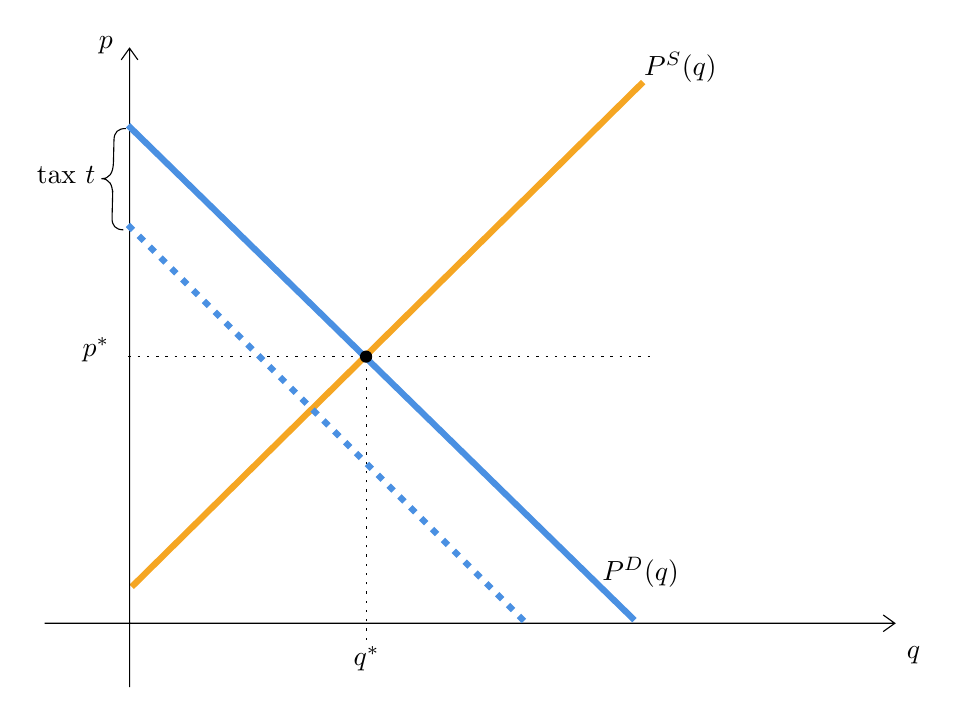
\begin{tikzpicture}[x=0.6pt,y=0.6pt,yscale=-1,xscale=1]
%uncomment if require: \path (0,443); %set diagram left start at 0, and has height of 443




%Supply
\draw [color={rgb, 255:red, 245; green, 166; blue, 35 }  ,draw opacity=1 ][line width=2.25]    (126.5,361) -- (434.5,57) ;


%AXES
\draw  (74,382.93) -- (586.09,382.93)(125.21,36.6) -- (125.21,421.41) (579.09,377.93) -- (586.09,382.93) -- (579.09,387.93) (120.21,43.6) -- (125.21,36.6) -- (130.21,43.6)  ;
Straight Lines [id:da1654344051931811] 
\draw [color={rgb, 255:red, 74; green, 144; blue, 226 }  ,draw opacity=1 ][line width=2.25]    (124.28,83.03) -- (429.28,381.03) ;


%Equilibrium Point
\draw  [draw opacity=0][fill={rgb, 255:red, 0; green, 0; blue, 0 }  ,fill opacity=1 ] (263.97,222.35) .. controls (263.97,220.32) and (265.61,218.67) .. (267.65,218.67) .. controls (269.68,218.67) and (271.33,220.32) .. (271.33,222.35) .. controls (271.33,224.39) and (269.68,226.03) .. (267.65,226.03) .. controls (265.61,226.03) and (263.97,224.39) .. (263.97,222.35) -- cycle ;

%Shifted Demand
\draw  [dash pattern={on 0.84pt off 2.51pt}]  (124.5,222) -- (441.5,222) ;


%Straight Lines: EQ quanitity
\draw  [dash pattern={on 0.84pt off 2.51pt}]  (267.65,393) -- (267.65,222.35) ;


%Consumer Surplus
% \draw  [draw opacity=0][fill={rgb, 255:red, 74; green, 144; blue, 226 }  ,fill opacity=0.15 ] (124.28,83.03) -- (263.97,222.35) -- (124.28,222.35) -- cycle ;

%Shape: Producer Surplus
%\draw  [draw opacity=0][fill={rgb, 255:red, 0; green, 0; blue, 0 }  ,fill opacity=0.5 ] (267.18,224.07) -- (234.08,254.31) -- (235.65,192) -- cycle ;

%Deadweight Loss
%\draw  [draw opacity=0][fill={rgb, 255:red, 245; green, 166; blue, 35 }  ,fill opacity=0.15 ] (124.43,363) -- (267.5,222.35) -- (124.43,222.35) -- cycle ; \draw    (270.5,153) -- (245,219) ;\draw (275,137) node  [align=left] {Deadweight Loss};



%Demand
\draw [color={rgb, 255:red, 74; green, 144; blue, 226 }  ,draw opacity=1 ][line width=2.25]  [dash pattern={on 2.53pt off 3.02pt}]  (124.28,143.03) -- (364.25,383) ;


%Straight Lines: Shifted EQ quantity
%\draw  [dash pattern={on 0.84pt off 2.51pt}]  (235.65,389) -- (235.65,254.35) ;
%\draw  [dash pattern={on 0.84pt off 2.51pt}]  (235.65,254.35) -- (235.65,192) ;

%Shifted Eq price: Consumer & Supplier
%\draw [shift={(235.65,192)}, rotate = 270] [color={rgb, 255:red, 0; green, 0; blue, 0 }  ][fill={rgb, 255:red, 0; green, 0; blue, 0 }  ][line width=0.75]      (0, 0) circle [x radius= 3.35, y radius= 3.35]   ;
%\draw [shift={(235.65,254.35)}, rotate = 270] [color={rgb, 255:red, 0; green, 0; blue, 0 }  ][fill={rgb, 255:red, 0; green, 0; blue, 0 }  ][line width=0.75]      (0, 0) circle [x radius= 3.35, y radius= 3.35]   ;

%Shape: Brace Taxes-- 
\draw   (123,85) .. controls (118.33,84.89) and (115.94,87.16) .. (115.83,91.83) -- (115.5,105.33) .. controls (115.33,112) and (112.92,115.27) .. (108.25,115.16) .. controls (112.92,115.27) and (115.17,118.66) .. (115.01,125.32)(115.08,122.33) -- (114.67,138.83) .. controls (114.56,143.5) and (116.83,145.89) .. (121.5,146) ;\draw (87,113) node   {$\text{tax} \ t$};

%Straight Lines: shifted Eq price, consumer -- \draw  [dash pattern={on 0.84pt off 2.51pt}]  (120.5,192) -- (235.65,192) ;


%Straight Lines:: shifted Eq price, producer
%\draw  [dash pattern={on 0.84pt off 2.51pt}]  (120.5,254.35) -- (235.65,254.35) ;



%Straight Lines [id:da5864491930417586] 




\draw (597.35,402.33) node   {$q$};
\draw (111,35) node   {$p$};
\draw (457,48) node   {$P^S(q)$};
\draw (433,352) node   {$P^D(q)$};
\draw (105,218) node   {$p^{*}$};
\draw (268,404) node   {$q^{*}$};
%\draw (236,409) node   {$\hat{q}$};
%\draw (104,187) node   {$\hat{p}_{c}$};
%\draw (107,266) node   {$\hat{p}_{f}$};
%


\end{tikzpicture}}




\only<3>{

\tikzset{every picture/.style={line width=0.75pt}} %set default line width to 0.75pt        

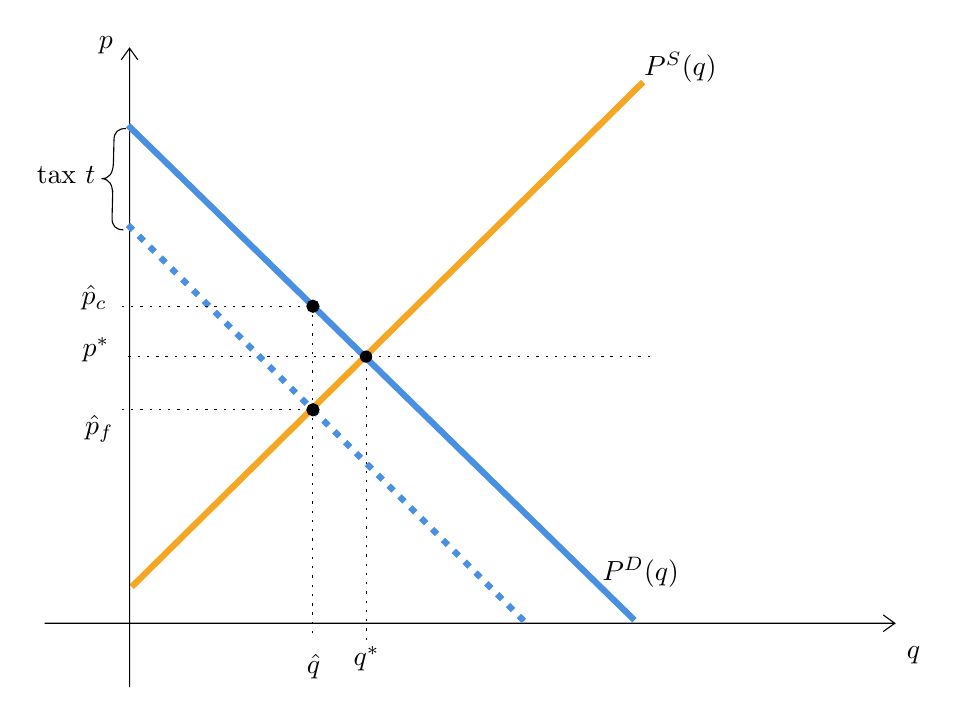
\begin{tikzpicture}[x=0.6pt,y=0.6pt,yscale=-1,xscale=1]
%uncomment if require: \path (0,443); %set diagram left start at 0, and has height of 443




%Supply
\draw [color={rgb, 255:red, 245; green, 166; blue, 35 }  ,draw opacity=1 ][line width=2.25]    (126.5,361) -- (434.5,57) ;


%AXES
\draw  (74,382.93) -- (586.09,382.93)(125.21,36.6) -- (125.21,421.41) (579.09,377.93) -- (586.09,382.93) -- (579.09,387.93) (120.21,43.6) -- (125.21,36.6) -- (130.21,43.6)  ;
Straight Lines [id:da1654344051931811] 
\draw [color={rgb, 255:red, 74; green, 144; blue, 226 }  ,draw opacity=1 ][line width=2.25]    (124.28,83.03) -- (429.28,381.03) ;


%Equilibrium Point
\draw  [draw opacity=0][fill={rgb, 255:red, 0; green, 0; blue, 0 }  ,fill opacity=1 ] (263.97,222.35) .. controls (263.97,220.32) and (265.61,218.67) .. (267.65,218.67) .. controls (269.68,218.67) and (271.33,220.32) .. (271.33,222.35) .. controls (271.33,224.39) and (269.68,226.03) .. (267.65,226.03) .. controls (265.61,226.03) and (263.97,224.39) .. (263.97,222.35) -- cycle ;

%Shifted Demand
\draw  [dash pattern={on 0.84pt off 2.51pt}]  (124.5,222) -- (441.5,222) ;


%Straight Lines: EQ quanitity
\draw  [dash pattern={on 0.84pt off 2.51pt}]  (267.65,393) -- (267.65,222.35) ;


%Consumer Surplus
% \draw  [draw opacity=0][fill={rgb, 255:red, 74; green, 144; blue, 226 }  ,fill opacity=0.15 ] (124.28,83.03) -- (263.97,222.35) -- (124.28,222.35) -- cycle ;

%Producer Surplus
%\draw  [draw opacity=0][fill={rgb, 255:red, 0; green, 0; blue, 0 }  ,fill opacity=0.5 ] (267.18,224.07) -- (234.08,254.31) -- (235.65,192) -- cycle ;

%Deadweight Loss
%\draw  [draw opacity=0][fill={rgb, 255:red, 245; green, 166; blue, 35 }  ,fill opacity=0.15 ] (124.43,363) -- (267.5,222.35) -- (124.43,222.35) -- cycle ; \draw    (270.5,153) -- (245,219) ;\draw (275,137) node  [align=left] {Deadweight Loss};



%Demand
\draw [color={rgb, 255:red, 74; green, 144; blue, 226 }  ,draw opacity=1 ][line width=2.25]  [dash pattern={on 2.53pt off 3.02pt}]  (124.28,143.03) -- (364.25,383) ;


%Straight Lines: Shifted EQ quantity
\draw  [dash pattern={on 0.84pt off 2.51pt}]  (235.65,389) -- (235.65,254.35) ;
\draw  [dash pattern={on 0.84pt off 2.51pt}]  (235.65,254.35) -- (235.65,192) ;

%Shifted Eq price Points: Consumer & Supplier
\draw [shift={(235.65,192)}, rotate = 270] [color={rgb, 255:red, 0; green, 0; blue, 0 }  ][fill={rgb, 255:red, 0; green, 0; blue, 0 }  ][line width=0.75]      (0, 0) circle [x radius= 3.35, y radius= 3.35]   ;
\draw [shift={(235.65,254.35)}, rotate = 270] [color={rgb, 255:red, 0; green, 0; blue, 0 }  ][fill={rgb, 255:red, 0; green, 0; blue, 0 }  ][line width=0.75]      (0, 0) circle [x radius= 3.35, y radius= 3.35]   ;

%Shape: Brace Taxes-- 
\draw   (123,85) .. controls (118.33,84.89) and (115.94,87.16) .. (115.83,91.83) -- (115.5,105.33) .. controls (115.33,112) and (112.92,115.27) .. (108.25,115.16) .. controls (112.92,115.27) and (115.17,118.66) .. (115.01,125.32)(115.08,122.33) -- (114.67,138.83) .. controls (114.56,143.5) and (116.83,145.89) .. (121.5,146) ;\draw (87,113) node   {$\text{tax} \ t$};

%Straight Lines: shifted Eq price, consumer & Producer 
\draw  [dash pattern={on 0.84pt off 2.51pt}]  (120.5,192) -- (235.65,192) ;
\draw  [dash pattern={on 0.84pt off 2.51pt}]  (120.5,254.35) -- (235.65,254.35) ;





%Straight Lines [id:da5864491930417586] 




\draw (597.35,402.33) node   {$q$};
\draw (111,35) node   {$p$};
\draw (457,48) node   {$P^S(q)$};
\draw (433,352) node   {$P^D(q)$};
\draw (105,218) node   {$p^{*}$};
\draw (268,404) node   {$q^{*}$};
\draw (236,409) node   {$\hat{q}$};
\draw (104,187) node   {$\hat{p}_{c}$};
\draw (107,266) node   {$\hat{p}_{f}$};
%


\end{tikzpicture}}




\only<4>{

\tikzset{every picture/.style={line width=0.75pt}} %set default line width to 0.75pt        

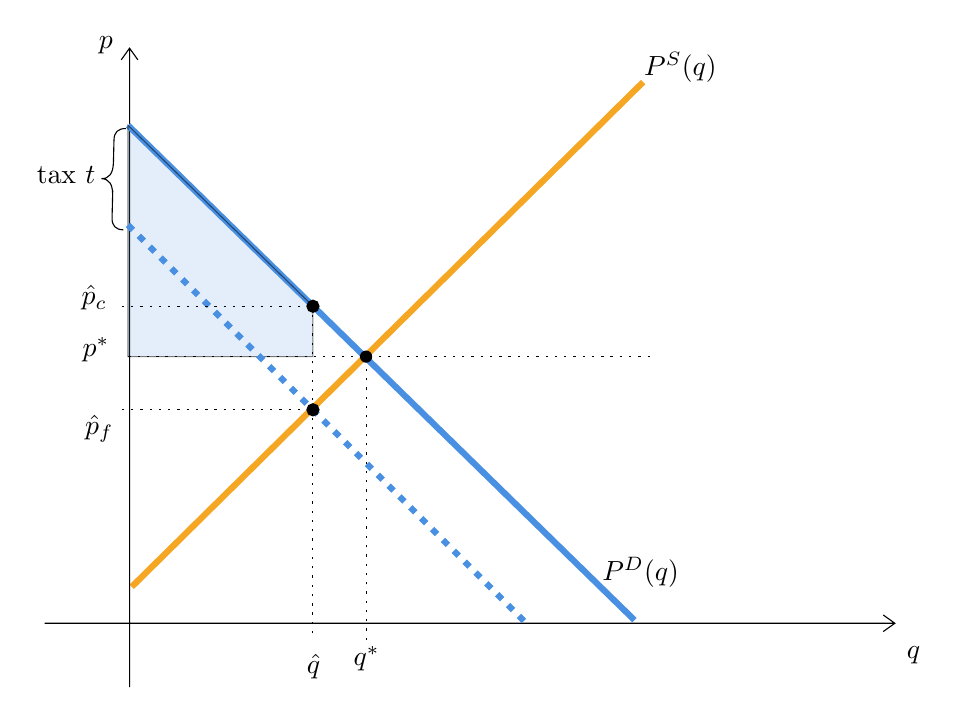
\begin{tikzpicture}[x=0.6pt,y=0.6pt,yscale=-1,xscale=1]
%uncomment if require: \path (0,443); %set diagram left start at 0, and has height of 443




%Supply
\draw [color={rgb, 255:red, 245; green, 166; blue, 35 }  ,draw opacity=1 ][line width=2.25]    (126.5,361) -- (434.5,57) ;


%AXES
\draw  (74,382.93) -- (586.09,382.93)(125.21,36.6) -- (125.21,421.41) (579.09,377.93) -- (586.09,382.93) -- (579.09,387.93) (120.21,43.6) -- (125.21,36.6) -- (130.21,43.6)  ;
Straight Lines [id:da1654344051931811] 
\draw [color={rgb, 255:red, 74; green, 144; blue, 226 }  ,draw opacity=1 ][line width=2.25]    (124.28,83.03) -- (429.28,381.03) ;


%Equilibrium Point
\draw  [draw opacity=0][fill={rgb, 255:red, 0; green, 0; blue, 0 }  ,fill opacity=1 ] (263.97,222.35) .. controls (263.97,220.32) and (265.61,218.67) .. (267.65,218.67) .. controls (269.68,218.67) and (271.33,220.32) .. (271.33,222.35) .. controls (271.33,224.39) and (269.68,226.03) .. (267.65,226.03) .. controls (265.61,226.03) and (263.97,224.39) .. (263.97,222.35) -- cycle ;

%Shifted Demand
\draw  [dash pattern={on 0.84pt off 2.51pt}]  (124.5,222) -- (441.5,222) ;


%Straight Lines: EQ quanitity
\draw  [dash pattern={on 0.84pt off 2.51pt}]  (267.65,393) -- (267.65,222.35) ;


%Consumer  Surplus
\draw  [draw opacity=0.5][fill={rgb, 255:red, 74; green, 144; blue, 226 }  ,fill opacity=0.15 ] (124.28,83.03) -- (235.65,192) -- (235.65,222.35) -- (124.28,222.35) -- cycle ;

%Producer Surplus
%\draw  [draw opacity=0.5][fill={rgb, 255:red, 245; green, 166; blue, 35 }  ,fill opacity=0.15 ] (124.43,363)  -- (235.65,254.31) -- (235.65,222.35) -- (124.43,222.35) -- cycle ;




%Deadweight Loss
%\draw  [draw opacity=0][fill={rgb, 255:red, 0; green, 0; blue, 0 }  ,fill opacity=0.5 ] (267.18,224.07) -- (235.65,254.31) -- (235.65,192) -- cycle ; \draw    (270.5,153) -- (245,219) ;\draw (275,137) node  [align=left] {Deadweight Loss};






%Demand
\draw [color={rgb, 255:red, 74; green, 144; blue, 226 }  ,draw opacity=1 ][line width=2.25]  [dash pattern={on 2.53pt off 3.02pt}]  (124.28,143.03) -- (364.25,383) ;


%Straight Lines: Shifted EQ quantity
\draw  [dash pattern={on 0.84pt off 2.51pt}]  (235.65,389) -- (235.65,254.35) ;
\draw  [dash pattern={on 0.84pt off 2.51pt}]  (235.65,254.35) -- (235.65,192) ;

%Shifted Eq price Points: Consumer & Supplier
\draw [shift={(235.65,192)}, rotate = 270] [color={rgb, 255:red, 0; green, 0; blue, 0 }  ][fill={rgb, 255:red, 0; green, 0; blue, 0 }  ][line width=0.75]      (0, 0) circle [x radius= 3.35, y radius= 3.35]   ;
\draw [shift={(235.65,254.35)}, rotate = 270] [color={rgb, 255:red, 0; green, 0; blue, 0 }  ][fill={rgb, 255:red, 0; green, 0; blue, 0 }  ][line width=0.75]      (0, 0) circle [x radius= 3.35, y radius= 3.35]   ;

%Shape: Brace Taxes-- 
\draw   (123,85) .. controls (118.33,84.89) and (115.94,87.16) .. (115.83,91.83) -- (115.5,105.33) .. controls (115.33,112) and (112.92,115.27) .. (108.25,115.16) .. controls (112.92,115.27) and (115.17,118.66) .. (115.01,125.32)(115.08,122.33) -- (114.67,138.83) .. controls (114.56,143.5) and (116.83,145.89) .. (121.5,146) ;\draw (87,113) node   {$\text{tax} \ t$};

%Straight Lines: shifted Eq price, consumer & Producer 
\draw  [dash pattern={on 0.84pt off 2.51pt}]  (120.5,192) -- (235.65,192) ;
\draw  [dash pattern={on 0.84pt off 2.51pt}]  (120.5,254.35) -- (235.65,254.35) ;





%Straight Lines [id:da5864491930417586] 




\draw (597.35,402.33) node   {$q$};
\draw (111,35) node   {$p$};
\draw (457,48) node   {$P^S(q)$};
\draw (433,352) node   {$P^D(q)$};
\draw (105,218) node   {$p^{*}$};
\draw (268,404) node   {$q^{*}$};
\draw (236,409) node   {$\hat{q}$};
\draw (104,187) node   {$\hat{p}_{c}$};
\draw (107,266) node   {$\hat{p}_{f}$};
%


\end{tikzpicture}}




\only<5>{

\tikzset{every picture/.style={line width=0.75pt}} %set default line width to 0.75pt        

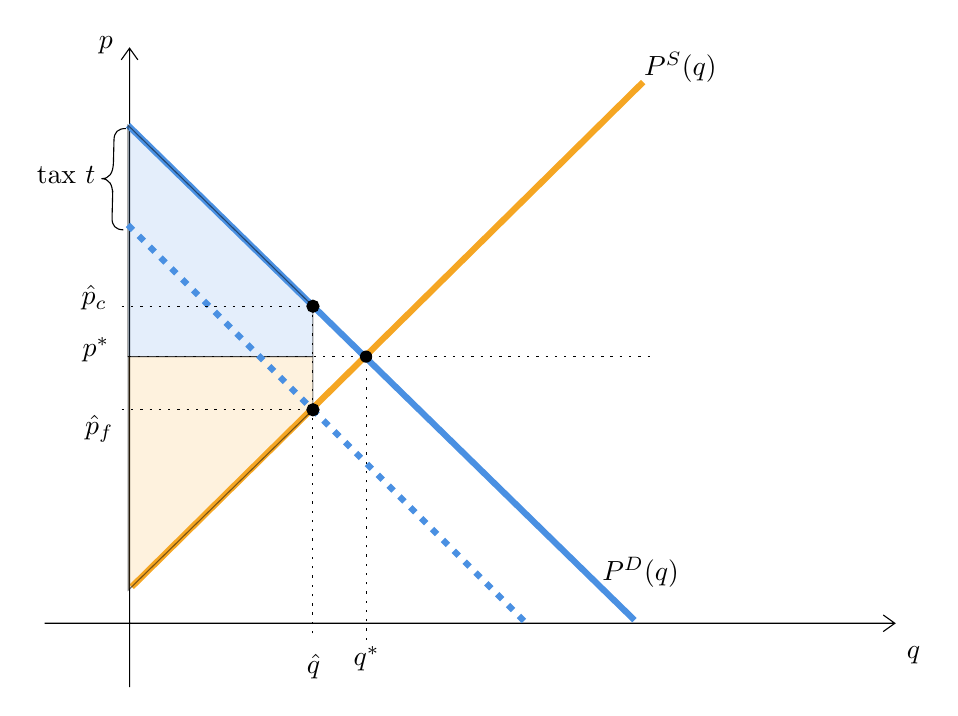
\begin{tikzpicture}[x=0.6pt,y=0.6pt,yscale=-1,xscale=1]
%uncomment if require: \path (0,443); %set diagram left start at 0, and has height of 443




%Supply
\draw [color={rgb, 255:red, 245; green, 166; blue, 35 }  ,draw opacity=1 ][line width=2.25]    (126.5,361) -- (434.5,57) ;


%AXES
\draw  (74,382.93) -- (586.09,382.93)(125.21,36.6) -- (125.21,421.41) (579.09,377.93) -- (586.09,382.93) -- (579.09,387.93) (120.21,43.6) -- (125.21,36.6) -- (130.21,43.6)  ;
Straight Lines [id:da1654344051931811] 
\draw [color={rgb, 255:red, 74; green, 144; blue, 226 }  ,draw opacity=1 ][line width=2.25]    (124.28,83.03) -- (429.28,381.03) ;


%Equilibrium Point
\draw  [draw opacity=0][fill={rgb, 255:red, 0; green, 0; blue, 0 }  ,fill opacity=1 ] (263.97,222.35) .. controls (263.97,220.32) and (265.61,218.67) .. (267.65,218.67) .. controls (269.68,218.67) and (271.33,220.32) .. (271.33,222.35) .. controls (271.33,224.39) and (269.68,226.03) .. (267.65,226.03) .. controls (265.61,226.03) and (263.97,224.39) .. (263.97,222.35) -- cycle ;

%Shifted Demand
\draw  [dash pattern={on 0.84pt off 2.51pt}]  (124.5,222) -- (441.5,222) ;


%Straight Lines: EQ quanitity
\draw  [dash pattern={on 0.84pt off 2.51pt}]  (267.65,393) -- (267.65,222.35) ;


%Consumer  Surplus
\draw  [draw opacity=0.5][fill={rgb, 255:red, 74; green, 144; blue, 226 }  ,fill opacity=0.15 ] (124.28,83.03) -- (235.65,192) -- (235.65,222.35) -- (124.28,222.35) -- cycle ;

%Producer Surplus
\draw  [draw opacity=0.5][fill={rgb, 255:red, 245; green, 166; blue, 35 }  ,fill opacity=0.15 ] (124.43,363)  -- (235.65,254.31) -- (235.65,222.35) -- (124.43,222.35) -- cycle ;




%Deadweight Loss
%\draw  [draw opacity=0][fill={rgb, 255:red, 0; green, 0; blue, 0 }  ,fill opacity=0.5 ] (267.18,224.07) -- (235.65,254.31) -- (235.65,192) -- cycle ; \draw    (270.5,153) -- (245,219) ;\draw (275,137) node  [align=left] {Deadweight Loss};






%Demand
\draw [color={rgb, 255:red, 74; green, 144; blue, 226 }  ,draw opacity=1 ][line width=2.25]  [dash pattern={on 2.53pt off 3.02pt}]  (124.28,143.03) -- (364.25,383) ;


%Straight Lines: Shifted EQ quantity
\draw  [dash pattern={on 0.84pt off 2.51pt}]  (235.65,389) -- (235.65,254.35) ;
\draw  [dash pattern={on 0.84pt off 2.51pt}]  (235.65,254.35) -- (235.65,192) ;

%Shifted Eq price Points: Consumer & Supplier
\draw [shift={(235.65,192)}, rotate = 270] [color={rgb, 255:red, 0; green, 0; blue, 0 }  ][fill={rgb, 255:red, 0; green, 0; blue, 0 }  ][line width=0.75]      (0, 0) circle [x radius= 3.35, y radius= 3.35]   ;
\draw [shift={(235.65,254.35)}, rotate = 270] [color={rgb, 255:red, 0; green, 0; blue, 0 }  ][fill={rgb, 255:red, 0; green, 0; blue, 0 }  ][line width=0.75]      (0, 0) circle [x radius= 3.35, y radius= 3.35]   ;

%Shape: Brace Taxes-- 
\draw   (123,85) .. controls (118.33,84.89) and (115.94,87.16) .. (115.83,91.83) -- (115.5,105.33) .. controls (115.33,112) and (112.92,115.27) .. (108.25,115.16) .. controls (112.92,115.27) and (115.17,118.66) .. (115.01,125.32)(115.08,122.33) -- (114.67,138.83) .. controls (114.56,143.5) and (116.83,145.89) .. (121.5,146) ;\draw (87,113) node   {$\text{tax} \ t$};

%Straight Lines: shifted Eq price, consumer & Producer 
\draw  [dash pattern={on 0.84pt off 2.51pt}]  (120.5,192) -- (235.65,192) ;
\draw  [dash pattern={on 0.84pt off 2.51pt}]  (120.5,254.35) -- (235.65,254.35) ;





%Straight Lines [id:da5864491930417586] 




\draw (597.35,402.33) node   {$q$};
\draw (111,35) node   {$p$};
\draw (457,48) node   {$P^S(q)$};
\draw (433,352) node   {$P^D(q)$};
\draw (105,218) node   {$p^{*}$};
\draw (268,404) node   {$q^{*}$};
\draw (236,409) node   {$\hat{q}$};
\draw (104,187) node   {$\hat{p}_{c}$};
\draw (107,266) node   {$\hat{p}_{f}$};
%


\end{tikzpicture}}




\only<6>{

\tikzset{every picture/.style={line width=0.75pt}} %set default line width to 0.75pt        

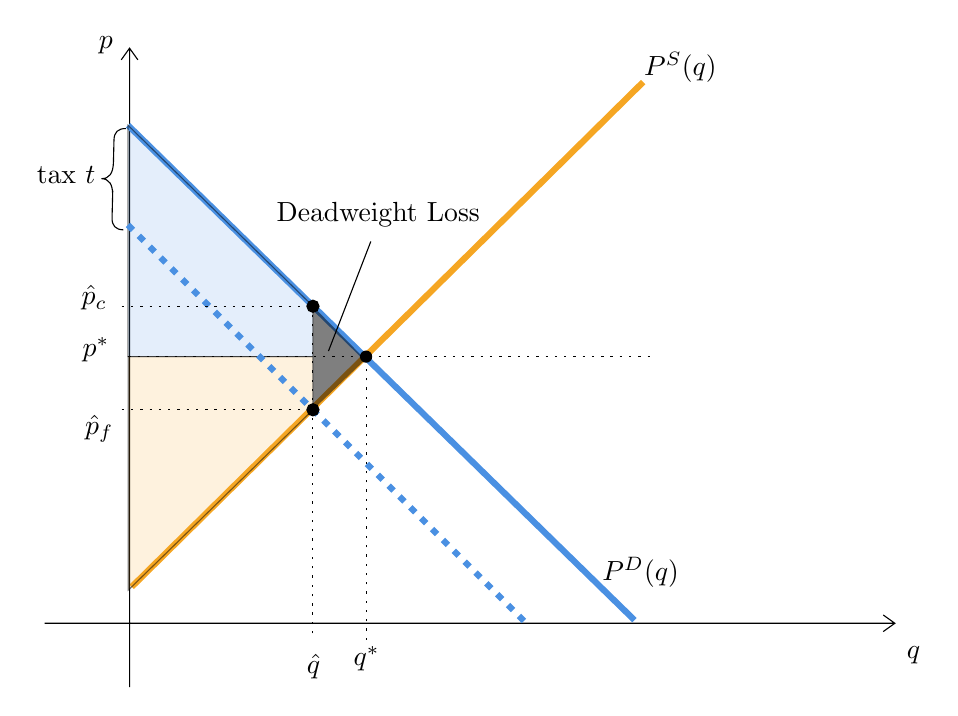
\begin{tikzpicture}[x=0.6pt,y=0.6pt,yscale=-1,xscale=1]
%uncomment if require: \path (0,443); %set diagram left start at 0, and has height of 443




%Supply
\draw [color={rgb, 255:red, 245; green, 166; blue, 35 }  ,draw opacity=1 ][line width=2.25]    (126.5,361) -- (434.5,57) ;


%AXES
\draw  (74,382.93) -- (586.09,382.93)(125.21,36.6) -- (125.21,421.41) (579.09,377.93) -- (586.09,382.93) -- (579.09,387.93) (120.21,43.6) -- (125.21,36.6) -- (130.21,43.6)  ;
Straight Lines [id:da1654344051931811] 
\draw [color={rgb, 255:red, 74; green, 144; blue, 226 }  ,draw opacity=1 ][line width=2.25]    (124.28,83.03) -- (429.28,381.03) ;


%Equilibrium Point
\draw  [draw opacity=0][fill={rgb, 255:red, 0; green, 0; blue, 0 }  ,fill opacity=1 ] (263.97,222.35) .. controls (263.97,220.32) and (265.61,218.67) .. (267.65,218.67) .. controls (269.68,218.67) and (271.33,220.32) .. (271.33,222.35) .. controls (271.33,224.39) and (269.68,226.03) .. (267.65,226.03) .. controls (265.61,226.03) and (263.97,224.39) .. (263.97,222.35) -- cycle ;

%Shifted Demand
\draw  [dash pattern={on 0.84pt off 2.51pt}]  (124.5,222) -- (441.5,222) ;


%Straight Lines: EQ quanitity
\draw  [dash pattern={on 0.84pt off 2.51pt}]  (267.65,393) -- (267.65,222.35) ;


%Consumer  Surplus
\draw  [draw opacity=0.5][fill={rgb, 255:red, 74; green, 144; blue, 226 }  ,fill opacity=0.15 ] (124.28,83.03) -- (235.65,192) -- (235.65,222.35) -- (124.28,222.35) -- cycle ;

%Producer Surplus
\draw  [draw opacity=0.5][fill={rgb, 255:red, 245; green, 166; blue, 35 }  ,fill opacity=0.15 ] (124.43,363)  -- (235.65,254.31) -- (235.65,222.35) -- (124.43,222.35) -- cycle ;




%Deadweight Loss
\draw  [draw opacity=0][fill={rgb, 255:red, 0; green, 0; blue, 0 }  ,fill opacity=0.5 ] (267.18,224.07) -- (235.65,254.31) -- (235.65,192) -- cycle ; \draw    (270.5,153) -- (245,219) ;\draw (275,137) node  [align=left] {Deadweight Loss};






%Demand
\draw [color={rgb, 255:red, 74; green, 144; blue, 226 }  ,draw opacity=1 ][line width=2.25]  [dash pattern={on 2.53pt off 3.02pt}]  (124.28,143.03) -- (364.25,383) ;


%Straight Lines: Shifted EQ quantity
\draw  [dash pattern={on 0.84pt off 2.51pt}]  (235.65,389) -- (235.65,254.35) ;
\draw  [dash pattern={on 0.84pt off 2.51pt}]  (235.65,254.35) -- (235.65,192) ;

%Shifted Eq price Points: Consumer & Supplier
\draw [shift={(235.65,192)}, rotate = 270] [color={rgb, 255:red, 0; green, 0; blue, 0 }  ][fill={rgb, 255:red, 0; green, 0; blue, 0 }  ][line width=0.75]      (0, 0) circle [x radius= 3.35, y radius= 3.35]   ;
\draw [shift={(235.65,254.35)}, rotate = 270] [color={rgb, 255:red, 0; green, 0; blue, 0 }  ][fill={rgb, 255:red, 0; green, 0; blue, 0 }  ][line width=0.75]      (0, 0) circle [x radius= 3.35, y radius= 3.35]   ;

%Shape: Brace Taxes-- 
\draw   (123,85) .. controls (118.33,84.89) and (115.94,87.16) .. (115.83,91.83) -- (115.5,105.33) .. controls (115.33,112) and (112.92,115.27) .. (108.25,115.16) .. controls (112.92,115.27) and (115.17,118.66) .. (115.01,125.32)(115.08,122.33) -- (114.67,138.83) .. controls (114.56,143.5) and (116.83,145.89) .. (121.5,146) ;\draw (87,113) node   {$\text{tax} \ t$};

%Straight Lines: shifted Eq price, consumer & Producer 
\draw  [dash pattern={on 0.84pt off 2.51pt}]  (120.5,192) -- (235.65,192) ;
\draw  [dash pattern={on 0.84pt off 2.51pt}]  (120.5,254.35) -- (235.65,254.35) ;





%Straight Lines [id:da5864491930417586] 




\draw (597.35,402.33) node   {$q$};
\draw (111,35) node   {$p$};
\draw (457,48) node   {$P^S(q)$};
\draw (433,352) node   {$P^D(q)$};
\draw (105,218) node   {$p^{*}$};
\draw (268,404) node   {$q^{*}$};
\draw (236,409) node   {$\hat{q}$};
\draw (104,187) node   {$\hat{p}_{c}$};
\draw (107,266) node   {$\hat{p}_{f}$};
%


\end{tikzpicture}}



\end{frame}
\end{document}